\subsection{Answer present}
At first, we had to decide which similarity algorithm to use when querying the database. 
To determine this, we queried all of our questions, containing only one word, to both indexes, and checked if the correct answers was present.
We did this for many number of passages, to see how the result evolved with increasing information.
We also ran this test using both Lucene default, and BM25 similarity, to determine which of these similarity algorithms that best suited our system.
The result can be seen in figure~\ref{fig:bm25_tfdf}.

\begin{figure}[h!]
  \centering
  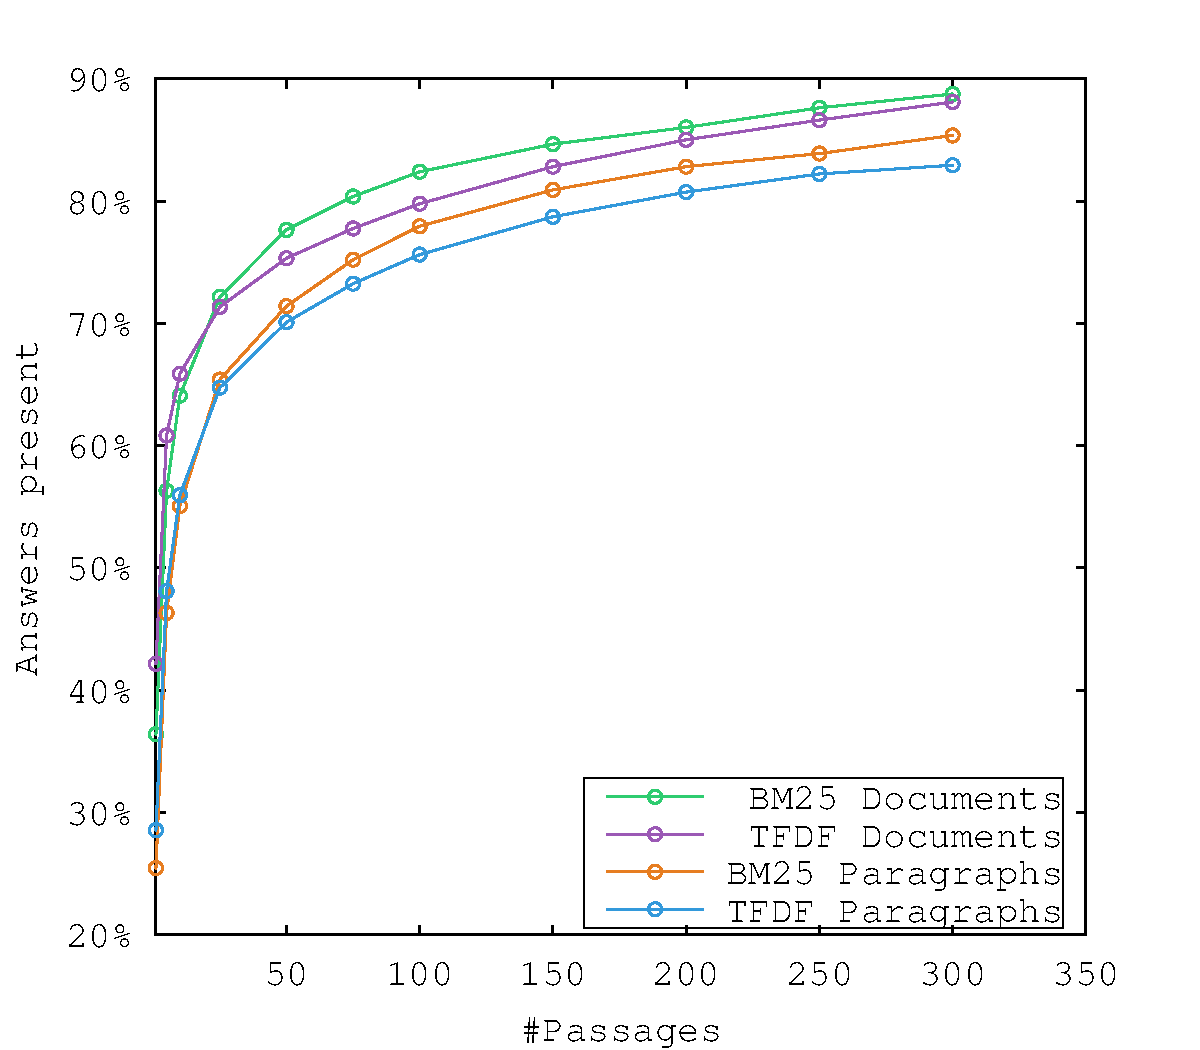
\includegraphics[width=0.5\textwidth]{figures/bm25_tfdf.pdf}
  \caption{Comparison between Lucene default, and BM25 similarities, when indexing by articles and paragraphs. 
  Shows how many percentages of the answers that were present for different number of passages.}
  \label{fig:bm25_tfdf}
\end{figure}

As we can see, BM25 is slightly better than Lucene default on all test with more than 25 passages, and no result can be 
considered acceptable using less than 25 passages.
Not surprisingly indexing by entire articles gives a better result than paragraphs, 
this can be explained by the fact that every article contains one or more paragraph. 
Which means that 100 article passages might yield the same amount of data as 200 paragraph passages.

\subsection{Noun extraction}

We needed to decide if we should index our wikipedia database dump by articles or paragraphs.
To decide this, we queried our two indexes, one indexed by paragraphs and
one indexed by articles, with all questions in our training set. We then extracted and 
ordered all nouns by frequency, and calculated the mean reciprocal rank (MRR). \cite{mrr}
If the answer was not present amongst the results, we disregarded the data point.
The result can be seen in figure~\ref{fig:median}.

\begin{figure}[h!]
  \centering
  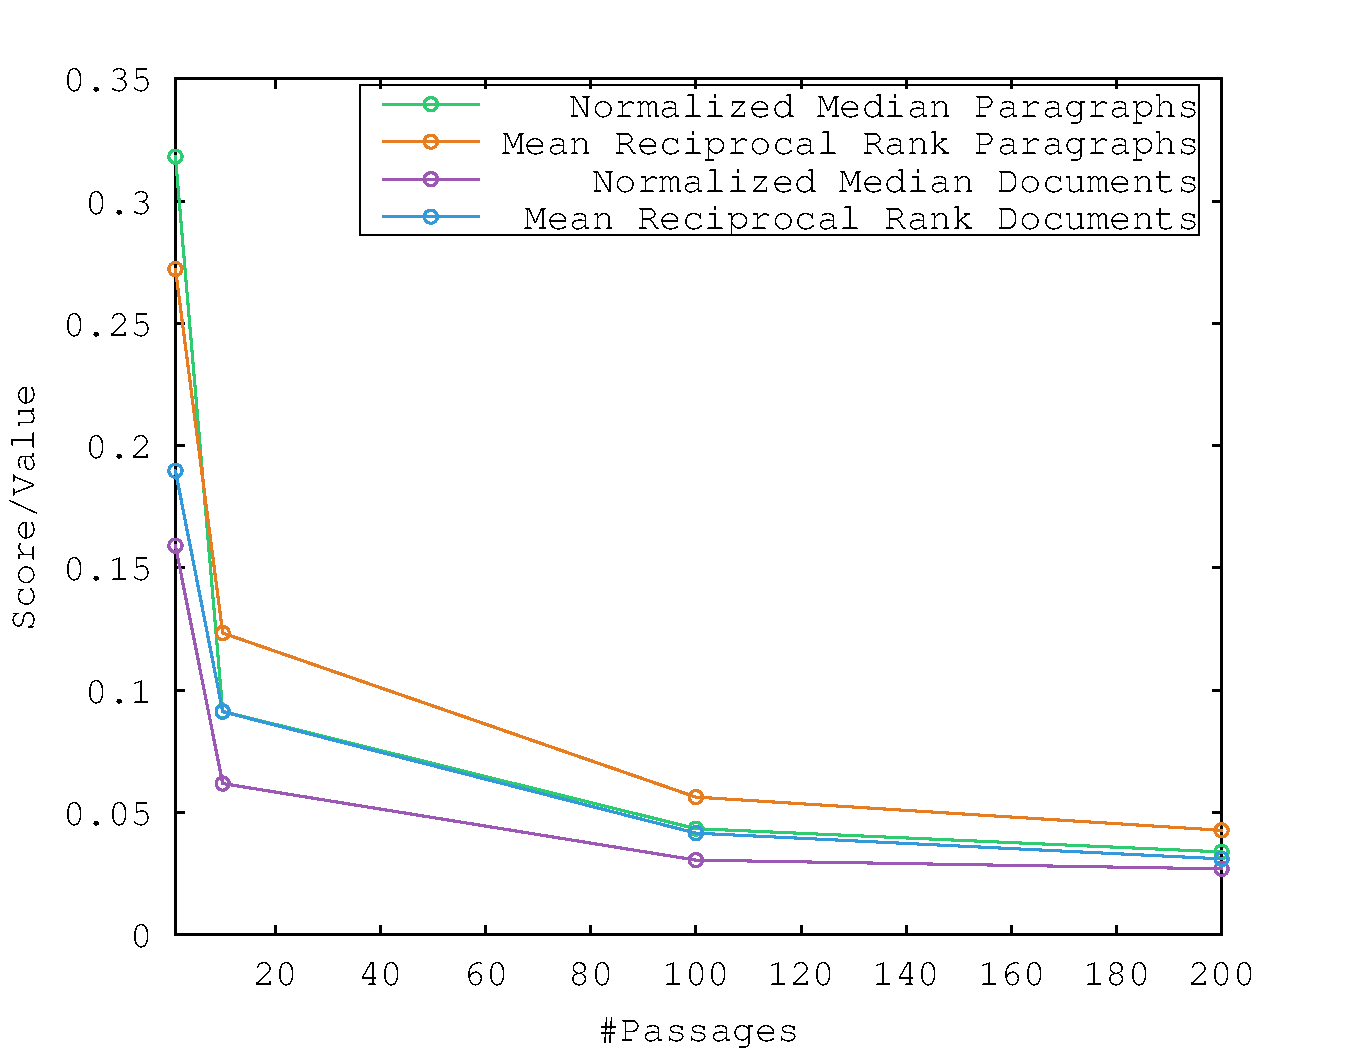
\includegraphics[width=0.5\textwidth]{figures/median.pdf}
  \caption{Comparison between indexing by articles, and indexing by paragraphs. 
  Shows the MRR values for the rank of the correct answer for the questions where 
  the answer is present.}
  \label{fig:median}
\end{figure}

As you can see, the mean reciprocal rank becomes lower as we extract more passages from the query, which
is natural since the frequency of frequently used swedish words increases as you increase the number
of passages extracted. Another phenomenon which we can observe is that the MRR for 
paragraphs is consistently higher than the MRR for documents, this is due to the amount of irrelevant
information contained in documents. Thus, the amount of relevant information is always more dense when
using a database indexed by paragraphs.

\subsection{Reranking}
Just extracting all nouns from the passages is not enough to acquire a valid answer, this is where the reranking comes in.
Using the trained model from all the questions, Liblinear is able to predict a probability that a specific noun is correct.
Combining this value with the value from Lucene, as mentioned, would increase the score of valid answers, and decrease the score of invalid ones.

Also, after reranking the answer candidates, there still exists some candidates that could be seen as impossible.
so using the puncher, as described, could in some cases improve the result further.

The result, measured using mean and median, can be seen in figure~\ref{fig:meanmedian}

\begin{figure}[h!]
  \centering
  \hspace*{-0.6cm}
  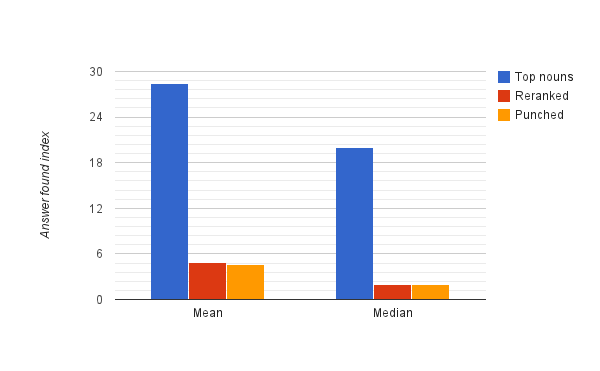
\includegraphics[width=0.6\textwidth]{figures/meanMedian.png}
  \caption{Comparison of answer ranks in the different stages of answer extraction.}
  \label{fig:meanmedian}
\end{figure}

The result, measured using MRR, can be seen in figure~\ref{fig:mrr}
\begin{figure}[h!]
  \centering
  \hspace*{-0.6cm}
  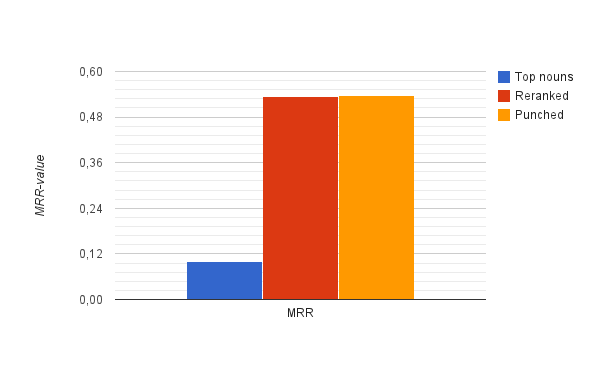
\includegraphics[width=0.6\textwidth]{figures/mrr.png}
  \caption{Comparison of answer ranks using MRR in the different stages of answer extraction.}
  \label{fig:mrr}
\end{figure}

As we can see, the reranking improves the result significantly, and the puncher gives a small boost.
By looking at the median values, we can see that for all the answers that are present, 
in half the cases the answer is located at the first or second place.
